\documentclass[10pt, a4paper]{article}
\usepackage[utf8]{inputenc}
\usepackage{fullpage}
\usepackage{amsmath,amsthm,amsfonts,amssymb,amscd}
\usepackage{lastpage}
\usepackage{enumerate}
\usepackage{fancyhdr}
\usepackage{mathrsfs}
\usepackage{xcolor}
\usepackage{graphicx}
\usepackage{listings}
\usepackage{preamble}
\usepackage{paralist}
\usepackage{ctable}
\usepackage{diagbox}
\usepackage{bm}
\usepackage{geometry}
\usepackage{float}
\usepackage{subfigure}
\usepackage{algorithm}
\usepackage{algorithmic}
\usepackage[colorlinks, linkcolor=blue]{hyperref}
\usepackage{animate}
\geometry{a4paper,scale=0.8}

\definecolor{codegreen}{rgb}{0,0.6,0}
\definecolor{codegray}{rgb}{0.5,0.5,0.5}
\definecolor{codepurple}{rgb}{0.58,0,0.82}
\definecolor{backcolour}{rgb}{0.95,0.95,0.92}

\lstdefinestyle{mystyle}{
    backgroundcolor=\color{backcolour},   
    commentstyle=\color{codegreen},
    keywordstyle=\color{magenta},
    numberstyle=\tiny\color{codegray},
    stringstyle=\color{codepurple},
    basicstyle=\ttfamily\footnotesize,
    breakatwhitespace=false,         
    breaklines=true,                 
    captionpos=b,                    
    keepspaces=true,                 
    numbers=left,                    
    numbersep=3pt,                  
    showspaces=false,                
    showstringspaces=false,
    showtabs=false,                  
    tabsize=2
}

\begin{document}
\section{Numerical Solution of PDE using PINN}
\subsection{Setting up the network}
We want to calculate the numerical solution of the following system of partial differential equations:

\begin{align*}
    \begin{cases}
        u_t-u_{xx} = f& \quad x\in (0,1) \text{ and } t\in(0,T)\\
        u(0,x)=\sin (2 \pi x)&\\
        u(t,0)= 0&\\
        u_x(t,1) = 2\pi e^{-t}&\\
    \end{cases}
\end{align*}

Its analytical solution is $u(t,x)=e^{-t}\sin(2\pi x)$ and $f=4e^{-t}\pi^2\sin(2\pi x)-e^{-t}\sin(2\pi x)$.

The general PINN structure for this equation is shown in figure \ref{fig:PINN}:

\begin{figure}[htbp!]
    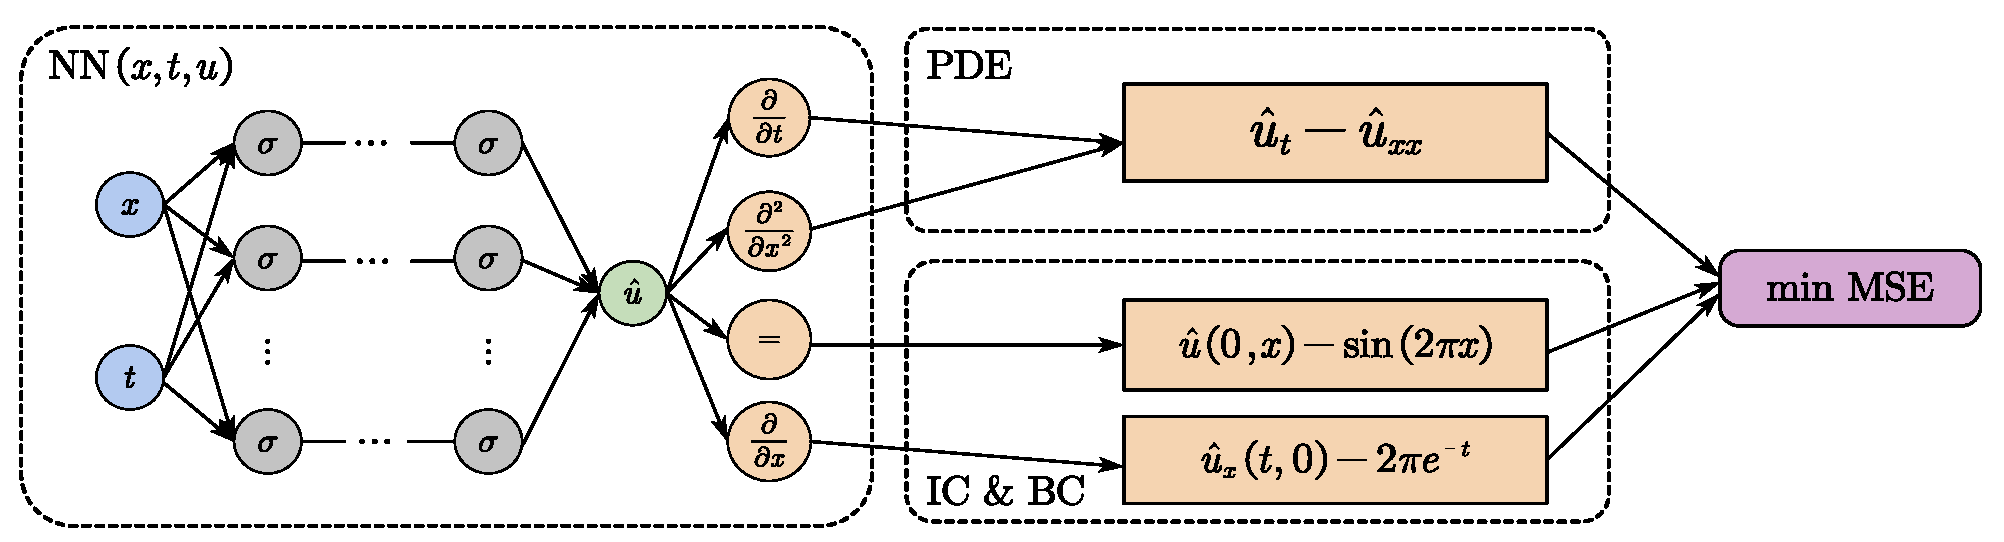
\includegraphics[width=\textwidth]{./pics/PINN.pdf}
    \caption{PINN consists of a neural network and loss calculation module.}
    \label{fig:PINN}
\end{figure}

The primary goal of PINN is to optimize the network by employing the starting values, boundary conditions, and equation definitions in the differential equations to cause the network to converge.
This is made possible by the automated differentiation mechanism offered by modern packages for neural network architecture.

Because of the simplicity of PyTorch's implementation of automatic differentiation and network structure, it is used to build the network structure. The implementation of neural network is shown in code snippet \ref{lst:nn}.

\lstset{style=mystyle}
\begin{lstlisting}[language=Python, caption=Definition of the neural network using PyTorch, label={lst:nn}]
import torch
import torch.nn as nn

class Wave(nn.Module):
    """
    Define the neural network,
    params: layer <int>, neurons <int>
    """

    def __init__(self, layer: int = 5, neurons: int = 20):
        # Input layer
        super(Wave, self).__init__()
        self.linear_in = nn.Linear(2, neurons)
        # Output layer
        self.linear_out = nn.Linear(neurons, 1)
        # Hidden Layers
        self.layers = nn.ModuleList(
            [nn.Linear(neurons, neurons) for i in range(layer)]
        )
        # Activation function
        self.act = nn.modules.Tanh()  # How about LeakyReLU? Or even Swish?

    def forward(self, x: torch.Tensor) -> torch.Tensor:
        x = self.linear_in(x)
        for layer in self.layers:
            x = self.act(layer(x))
        x = self.linear_out(x)
        return x
\end{lstlisting}


Let us define $f:=u_t-u_{xx}$.  $f$ can be simply defined in PyTorch as in code snippet \ref{lst:f}. Notice that in PyTorch, it is able to calculate high order derivatives by repeatedly using \lstinline{torch.autograd.grad}.


\begin{lstlisting}[language=Python, caption=Definition of the output using PyTorch, label={lst:f}]
def f(model, x_f, t_f, u_f):
    """
    This function evaluates the PDE at collocation points.
    """
    u = model(torch.stack((x_f, t_f), axis=1))[:, 0]  # Concatenates a seq of tensors along a new dimension
    u_t = derivative(u, t_f, order=1)
    u_xx = derivative(u, x_f, order=2)
    return u_t - u_xx - u_f

def derivative(dy: torch.Tensor, x: torch.Tensor, order: int = 1) -> torch.Tensor:
    """
    This function calculates the derivative of the model at x_f
    """
    for i in range(order):
        dy = torch.autograd.grad(
            dy, x, grad_outputs=torch.ones_like(dy), create_graph=True, retain_graph=True)[0]
    return 
\end{lstlisting}

We use MSE to measure the error. Define $\text{MSE}_{ic}$, $\text{MSE}_{bc}$ and $\text{MSE}_f$ for initial condition, boundary condition and collocation points, respectively.

The shared parameters between the neural networks $u(t,x)$ and $f(t,x)$ can be learned by minimizing the mean squared error loss
\[\text{MSE}=\text{MSE}_{f}+\text{MSE}_{ic}+\text{MSE}_{bc},\]
where \[\text{MSE}_f=\frac{1}{N_f}\sum_{i=1}^{N_f}\left|f(t^i,x^i)\right|^2,\]
and \[\begin{cases}
    \text{MSE}_{ic}=\frac{1}{N_{ic}}\sum_{i=1}^{N_{ic}}\left|u(t^i,x^i)-u\right|^2\\
    \text{MSE}_{bc}=\frac{1}{N_{bc}}\sum_{i=1}^{N_{bc}}\left|u(t^i,x^i)-u\right|^2\\
\end{cases}\]

Correspondingly, MSEs are implemented in PyTorch in code snippet \ref{lst:mse}.
\begin{lstlisting}[language=Python, caption=Definition of MSEs using PyTorch, label={lst:mse}]
def mse_f(model, x_f, t_f, u_f):
    """
    This function calculates the MSE for the PDE.
    """
    f_u = f(model, x_f, t_f, u_f)
    return (f_u ** 2).mean()


def mse_ic(model, x_ic, t_ic, u_ic):
    """
    This function calculates the MSE for the initial condition.
    u_ic is the real values
    """
    u = model(torch.stack((x_ic, t_ic), axis=1))[:, 0]
    return ((u - u_ic) ** 2).mean()


def mse_bc(model, l_t_bc, u_t_bc):
    """
    This function calculates the MSE for the boundary condition.
    """
    l_x_bc = torch.zeros_like(l_t_bc)
    l_x_bc.requires_grad = True
    l_u_bc = model(torch.stack((l_x_bc, l_t_bc), axis = 1))[:, 0]
    mse_dirichlet = (l_u_bc ** 2).mean()

    u_x_bc = torch.ones_like(u_t_bc)
    u_x_bc.requires_grad = True
    u_u_bc = model(torch.stack((u_x_bc, u_t_bc), axis=1))[:, 0]
    u_x_b_upper = derivative(u_u_bc, u_x_bc, 1)
    mse_neumann = (((2 * np.pi * torch.exp(-u_t_bc)) - u_x_b_upper) ** 2).mean()
    return mse_dirichlet + mse_neumann
\end{lstlisting}

The default hyper parameters are listed in table \ref{table:hp1}.

\ctable[pos=tbph,
label=table:hp1,
mincapwidth = 50mm,
caption = Settings of hyper parameters.
]{c|c}
{\tnote[a]{The learning rate is for LBFGS.}}
{
    \hline
    Hyper parameter &   value\\
    \hline
    \# Hidden layer  &   6\\
    \# Neurons per layer &   50\\
    \# Initial \& boundary points &   50\\
    \# Collocation points    &   9000\\
    \# epochs    &   1000\\
    \# Learning rate\tmark[a] &   1\\
    Optimization method &   LBFGS\\
    Activation function &   Tanh\\
    \hline
}

\subsection{Getting the prediction}

Figure \ref{fig:solwithpts} and \ref{fig:slice} show the predicted solution of this equation under the hyper-parameters in Table \ref{table:hp1}.


\begin{figure}[htb]
    \makebox[\textwidth][c]{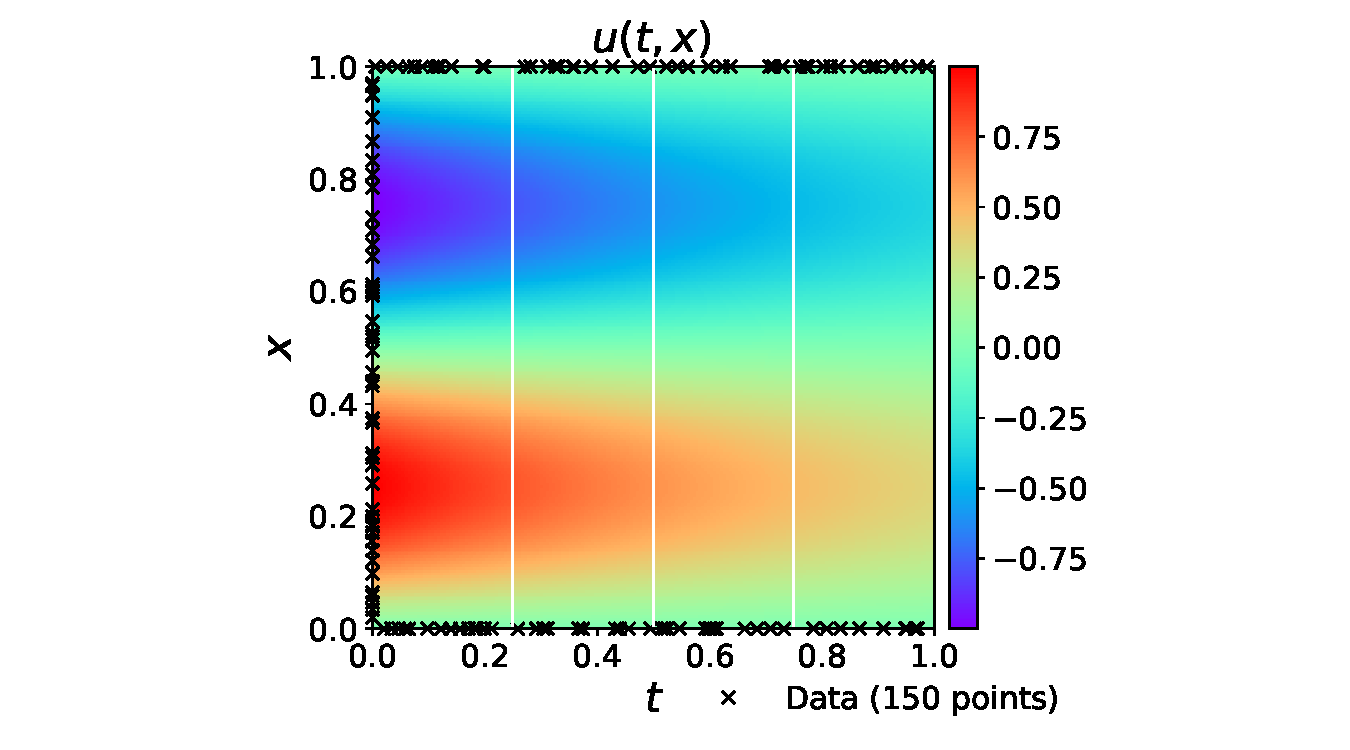
\includegraphics[width=\textwidth]{./pics/sol_with_point.pdf}}
    \caption{Predicted solution $u(t,x)$ along with the initial and boundary training data. The relative $\bb{L}_2 $ error for this case is $1.04\tms 10^{-3}$. Model training took 21.71s with 1000 epochs.}
    \label{fig:solwithpts}
\end{figure}

\clearpage

\begin{figure}[tbh]
\makebox[\textwidth][c]{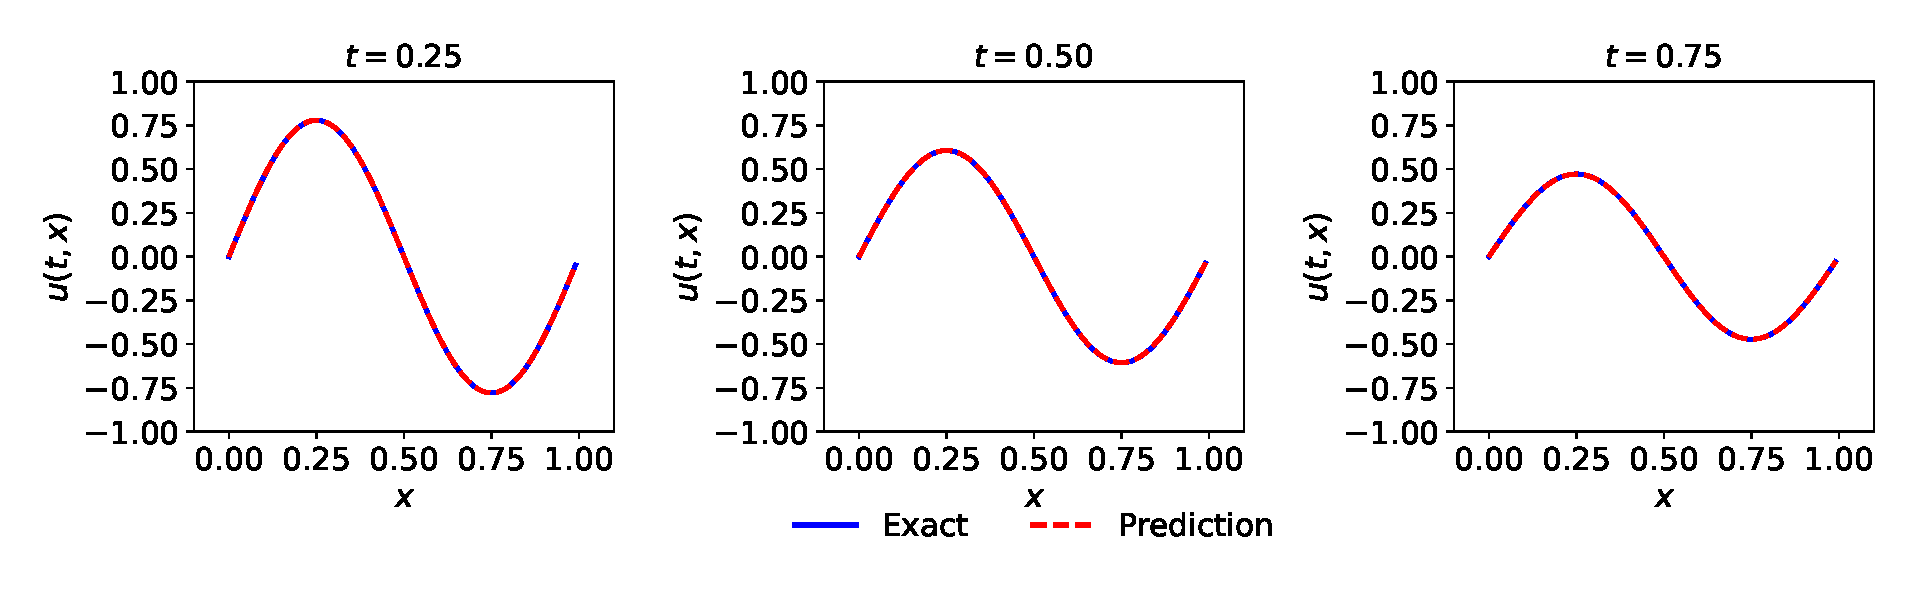
\includegraphics[width=1.1\textwidth]{./pics/slices.pdf}}
\caption{Comparison of the predicted and exact solution corresponding the the three temporal slices depicted by the white vertical lines in Figure \ref{fig:solwithpts}.}
\label{fig:slice}
\end{figure}

The errors are shown in Figure \ref{fig:error}.

\begin{figure}[th]
    \makebox[\textwidth][c]{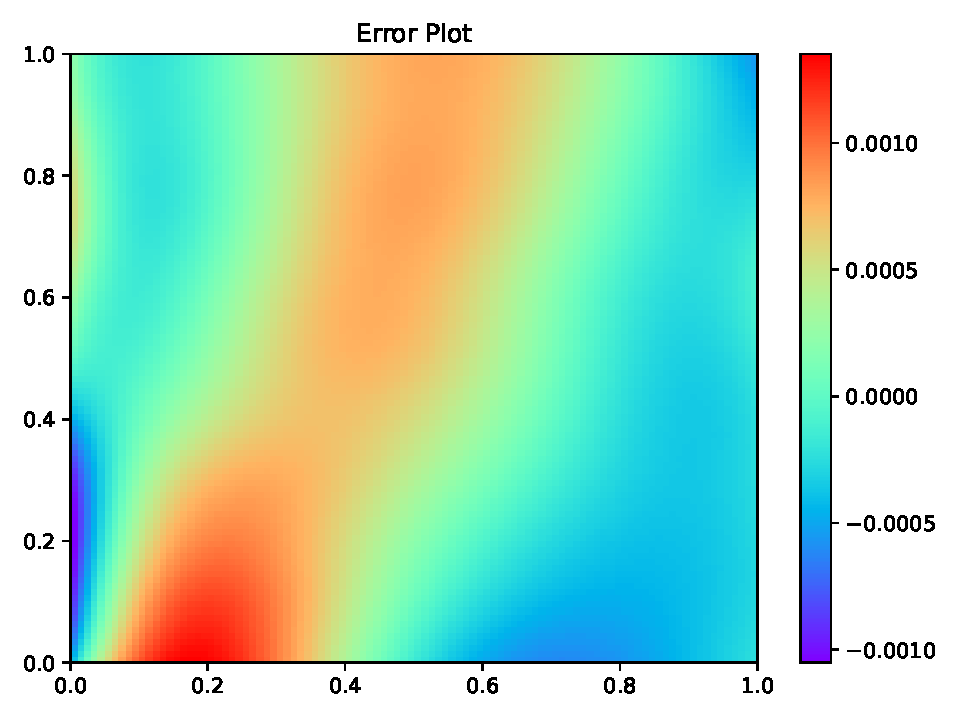
\includegraphics[width=0.45\textwidth]{./pics/error.pdf}}
    \caption{Error between the predicted and exact solution.}
    \label{fig:error}
\end{figure}


\begin{center}
    \animategraphics[loop,controls,width=0.5\linewidth]{5}{./outputpics/pic-}{1}{28}
\end{center}
\begin{center}
    Animation only available in Adobe Acrobat.
\end{center}

\newpage
\subsection{Investigation of hyper-parameters}

The investigated parameters are listed below:
\begin{compactenum}
    \item [Network Structure:]~
    \begin{compactenum}
        \item Number of layers
        \item Neurons per layer 
    \end{compactenum}
    \item [Optimization:]~
    \begin{compactenum}
        \item Optimization method: LBFGS, Adam, Ada, SGD, RMSProp
        \item Activation function: Tanh, GeLU, Mish, SoftPlus
    \end{compactenum}
    \item[Data:]~
    \begin{compactenum}
        \item Points on initial condition
        \item Points on boundary condition
        \item Collocation points
    \end{compactenum}
\end{compactenum}

We shall check the relative $\bb{L}_2$ by varying these hyper-parameters and record them using TensorBoard.

Table \ref{tbl:nn} gives the relative error $\bb{L}_2$ between the predicted and the exact solution using different number of hidden layers (2, 4, 6, 8, 10) and neurons per hidden layer (10, 30, 50, 70, 90). The optimal scheme is 6 hidden layer and 90 neurons with relative error of 0.046\% and loss of $9.6\tms 10^{-6}$.

\ctable[pos=tbph,
mincapwidth = 80mm,
caption = Relative error (\%) and loss ($10^{-4}$) between the predicted and the exact solution under different number of hidden layers $N_l$ and neurons per layer $N_n$.,
label={tbl:nn}
]{c|ccccc}
{
\tnote[]{$N_i=100$, $N_c=5000$, epoch=1000 and lr=1, using LBFGS.}
\tnote[a]{The result are show in the form \textit{error\ }(\textit{loss})}
\tnote[b]{The smallest error are in bold font.}
}
{
\hline
\diagbox{$N_n$}{$N_l$}  & 2     & 4     & 6     & 8     & 10    \\ \hline
 10 & 0.846\ (6.779)\tmark[a] & 0.664\ (6.508)& 1.079\ (6.660)& 4.328\ (72.123)& 4.512\ (239.600)\\
 30 & 0.258\ (4.110)& 0.245\ (1.115)& 0.300\ (1.234)& 0.297\ (2.922)& 0.255\ (1.347)\\
 50 & 0.252\ (2.183)& 0.176\ (1.156)& 0.238\ (1.550)& 0.128\ (1.916)& 0.279\ (4.296)\\
 70 & 0.249\ (3.240)& 0.104\ (0.328)& 0.088\ (0.437)& 0.242\ (0.736)& 0.199\ (0.698)\\
 90 & 0.581\ (3.865)& 0.335\ (1.084)& \textbf{0.046}\ (\textbf{0.096})\tmark[b]& 0.155\ (0.158)& 0.112\ (0.460)\\ \hline
}

Table \ref{tbl: data} gives the relative error by varying the number of initial,(each) boundary points (30, 40, 50, 60, 70) and collocation points (1000, 3000, 5000, 7000, 9000). The optimal scheme for minimizing relative error is 30 initial points, 60 boundary points (a total of 90 points) and 9000 collocation points with relative error of 0.038\% and loss of $2.142\tms 10^{-5}$ while for minimizing loss is 70 initial points, 140 boundary points (a total of 210 points) and 3000 collocation points with relative error of 0.1\% and loss of $1.339\tms 10^{-5}$.

\ctable[pos=tbph,
mincapwidth = 80mm,
caption = Relative error (\%) and loss ($10^{-5}$) between the predicted and the exact solution under different number of initial and boundary points $N_i$ and collocation points $N_c$.,
label= {tbl: data}
]{c|ccccc}
{
\tnote[]{$N_l=4$, $N_n=40$, epoch=1000 and lr=1, using LBFGS.}}
{
    \hline
    \diagbox{$N_i$}{$N_c$} & 30     & 40     & 50     & 60     & 70     \\ 
    \hline
    1000 & 0.084\ (5.104)& 0.095\ (2.393)& 0.150\ (4.968)& 0.085\ (1.845)& 0.065\ (2.257)\\
    3000 & 0.090\ (2.666)& 0.246\ (2.942)& 0.087\ (2.396)& 0.211\ (3.664)& 0.100\ (\textbf{1.339})\\
    5000 & 0.185\ (3.591)& 0.100\ (2.502)& 0.051\ (1.644)& 0.173\ (5.367)& 0.114\ (2.311)\\
    7000 & 0.163\ (4.331)& 0.185\ (2.108)& 0.173\ (3.111)& 0.197\ (4.339)& 0.082\ (2.638)\\
    9000 & \textbf{0.038}\ (2.142)& 0.133\ (2.194)& 0.121\ (2.546)& 0.049\ (1.994)& 0.159\ (3.470)\\
    \hline
}

Table \ref{tbl:lr} gives the relative error by changing the learning epochs (500, 750, 1000, 1250, 1500) and learning rate (0.01, 0.1, 0.5, 0.1, 2, 5). The optimal schemes are found when learning rate is 1 and epoch are 1250 or 1500 with relative error of 0.02\% and loss of $1.280\tms 10^{-5}$.
\clearpage

\ctable[pos=!h,
mincapwidth = 100mm,
caption = Relative error (\%) and loss ($10^{-4}$) between the predicted and the exact solution under different epochs $E$ and learning rate.,
label = {tbl:lr}
]{c|cccccc}
{
\tnote[]{$N_l=6$, $N_n=50$, $N_i=50$ and $N_c=9000$, using LBFGS.}
\tnote[a]{Both are smallest.}
}
{
    \hline
\diagbox{$E$}{lr} & 0.01  & 0.1   & 0.5   & 1     & 2     & 5     \\ \hline
500  & 2.407\ (50.059)& 0.987\ (12.172)& 0.404\ (8.446)& 0.192\ (0.842)& 0.283\ (4.592)& 0.279\ (2.868)\\
750  & 1.052\ (16.980)& 0.441\ (2.743)& 0.125\ (1.866)& 0.077\ (0.316)& 0.149\ (2.477)& 0.286\ (1.159)\\
1000 & 0.722\ (5.912)& 0.276\ (1.345)& 0.125\ (0.634)& 0.051\ (0.164)& 0.139\ (2.078)& 0.222\ (0.557)\\
1250 & 0.441\ (3.648)& 0.240\ (1.017)& 0.081\ (0.337)& \textbf{0.020}\ (\textbf{0.128})\tmark[a]& 0.192\ (1.391)& 0.216\ (0.301)\\
1500 & 0.494\ (2.457)& 0.204\ (0.839)& 0.076\ (0.166)& \textbf{0.020}\ (\textbf{0.128})\tmark[a]& 0.134\ (0.954)& 0.195\ (0.244)\\ \hline
}




Then, as shown in Table \ref{tbl:method} and Figure \ref{fig:method}, we investigated the impact of several optimization methods on convergence speed and final error. In terms of convergence speed and final error, the second-order method L-BFGS offers an advantage over alternative first-order methods. \cite{lbfgs} It is worth noting that first-order algorithms, like Adam, are effective of performing error-insensitive computations.

\ctable[pos=!h,
mincapwidth = 100mm,
caption = Final loss and error (\%) between the predicted and the exact solution using different optimization methods,
label = {tbl:method}
]{c|ccccc}
{
\tnote[]{$N_l=6$, $N_n=50$, $N_i=50$ and $N_c=9000$, using Tanh.}}
{
\hline
\diagbox{Attribute}{Opt. Method}     & L-BFGS  & SGD   & Ada   & RMSProp & Adam \\ \hline
Loss  & $\bf{3.315}\tms \bf{10}^{\bf{-5}}$ & 2.656 & 0.140 & $7.48\tms 10^{-2}$ & 0.223\\
Rel. Error  & \textbf{0.105} & 147.430 & 6.352 & 17.950 & 7.596  \\
\hline
}

\begin{figure}[th]
    \makebox[\textwidth][c]{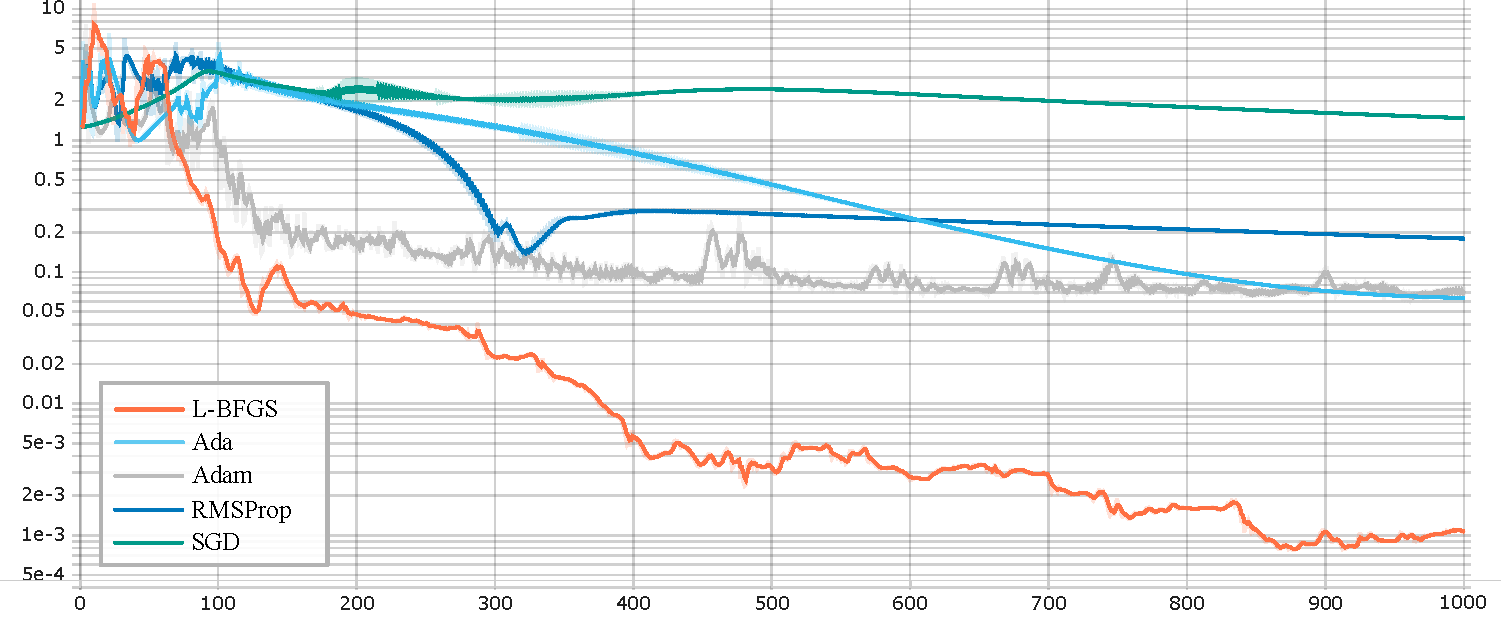
\includegraphics[width=\textwidth]{./pics/method.pdf}}
    \caption{Relative error using different Optimization method. L-BFGS outperforms among other optimization algorithms.}
    \label{fig:method}
\end{figure}

Finally, as seen in Table \ref{tbl:act} and Figure \ref{fig:act}, we study the convergence rate and final error/loss using various activation functions with default settings. According to the results, Mish has the fastest convergence and best relative error and Tanh has smallest loss comparing to other activation functions. On other tasks, Mish generally outperforms than other activation functions. \cite{mish}

\begin{figure}[!h]
    \makebox[\textwidth][c]{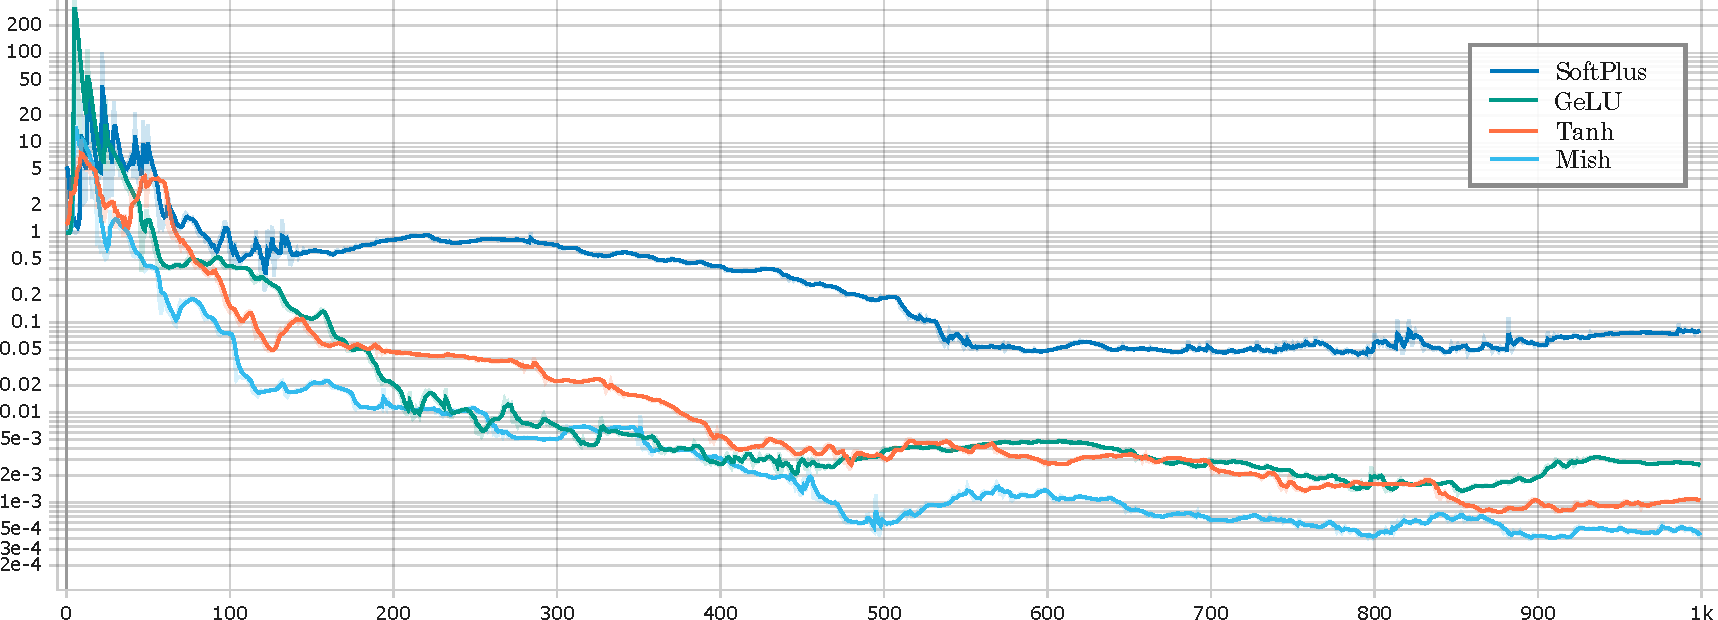
\includegraphics[width=\textwidth]{./pics/act.pdf}}
    \caption{Relative error under different activation functions. Mish outperforms among other activation functions.}
    \label{fig:act}
\end{figure}

\ctable[pos=!h,
mincapwidth = 100mm,
caption = Final loss and error (\%) between the predicted and the exact solution using different activation functions,
label = {tbl:act}
]{c|cccc}
{
\tnote[]{$N_l=6$, $N_n=50$, $N_i=50$ and $N_c=9000$, using LBFGS.}}
{
\hline
\diagbox{Attribute}{Act. Func.}     & Tanh  & GeLU   & Mish   & SoftPlus \\ \hline
Loss  & $\bf{3.315}\tms \bf{10}^{\bf{-5}}$ & $8.267\tms 10^{-5}$ & $3.433\tms 10^{-5}$ & $7.484\tms 10^{-2}$ \\
Rel. Error  & 0.105 & 0.255 & \textbf{0.0490} & 8.303  \\
\hline
}

\newpage

\subsection{Codes}

All the code using for this report can be found in the next url: \url{https://github.com/BeteixZ/PINN_from_beginning}.

    Le, Quoc V., et al. On optimization methods for deep learning. \textit{Proceedings of the 28th international conference on international conference on machine learning.} 2011.
	\bibitem{mish}
    Misra, Diganta. Mish: A self regularized non-monotonic activation function. \textit{arXiv preprint arXiv:1908.08681} 2020.



    
\end{thebibliography}

\end{document}